\documentclass[presentation, shownotes]{beamer}
\setbeamercovered{transparent}

\mode<presentation> {
    \usetheme{Frankfurt}
    \usecolortheme{whale}
    \setbeamertemplate{navigation symbols}{} % remove nav symbols
}

\usepackage[T1]{fontenc}
\usepackage[ngerman]{babel}
\usepackage[utf8]{inputenc}
\usepackage{graphicx}
\usepackage{booktabs}
\usepackage{listings}
\usepackage[
    backend=biber,
    style=authoryear,
    sorting=nyt,
    citestyle=authoryear]{biblatex}
\addbibresource{Literatur.bib}
\usepackage{csquotes}
\usepackage{relsize}

% make 'u.a.' 'et al.'
\DefineBibliographyStrings{ngerman}{
    andothers = {{et\,al\adddot}},
}

\graphicspath {{figures/}}

\def\ifmonospace{\ifdim\fontdimen3\font=0pt }

% prettier C++ formatting
\def\C++{%
\ifmonospace%
    C++%
\else%
    C\kern-.1667em\raise.30ex\hbox{\smaller{++}}%
\fi%
\spacefactor1000 }

%------------------------------------------------
%    TITLE PAGE
%------------------------------------------------

\title[Haskell vs. C++]{Vergleich paralleler Datenverarbeitung in Haskell und C++ anhand eines MapReduce Szenarios}

\author{Hans Christian Rudolph}
\institute[HfTL] {
    Hochschule für Telekommunikation Leipzig\\
    \medskip
    \textit{hans-christian.rudolph@hft-leipzig.de}\\
    \smallskip
    \textit{@hcrudolph}
}
\date{12. Oktober 2016}

\begin{document}

\begin{frame}
    \titlepage
\end{frame}

\begin{frame}[plain]{}
\begin{figure}
\centering
    \huge{
        \href{https://github.com/hcrudolph/oklab-parallel}{github.com/hcrudolph/oklab-parallel}
    }
\end{figure}
\end{frame}

\begin{frame}
    \frametitle{Gliederung}
    \tableofcontents
\end{frame}

%------------------------------------------------
%    BEGIN SLIDES
%-----------------------------------------------

%------------------------------------------------
\section{Einleitung}
\setcounter{subsection}{1}
%------------------------------------------------

\begin{frame}
\frametitle{Funktional vs. Imperativ}
\begin{columns}[c]
\column{.5\textwidth}
    \textbf{Haskell}
    \begin{itemize}
    \setlength\itemsep{1em}
    \item Rein funktional
    \item Stark abstrahiert
    \item Referenzielle Transparenz
    \end{itemize}

\column{.5\textwidth}
    \textbf{\C++}
    \begin{itemize}
    \setlength\itemsep{1em}
    \item Multiple Paradigmen
    \item (Wenn nötig) hardwarenah
    \item Zero-Cost Abstractions
    \end{itemize}
\end{columns}
\end{frame}

\begin{frame}[plain]{}
\begin{figure}
\centering

\includegraphics[height=.7\textheight]{parallel}
\end{figure}
\end{frame}

\begin{frame}
    \centering
    \citeauthor{marlow2009runtime} (\citeyear{marlow2009runtime}, S.1) stellen fest:\\ \bigskip
    \Large{
        ,,Plenty of papers describe promising ideas,\\ but vastly fewer describe real implementations [\dots]''.
    }
\end{frame}

\begin{frame}[plain]{}
\begin{figure}
\centering

\includegraphics[height=.7\textheight]{sad}
\end{figure}
\end{frame}

\begin{frame}
\frametitle{Begriffserklärung}

\pause

\onslide<2->{
\begin{block}{Nebenläufigkeit}
    beschreibt die unabhängige Ausführung von Berechnungen. Dies kann sowohl auf paralleler Hardware (mehrere CPUs) als auch auf sequenzieller geschehen.
    Es ist somit nicht ausgeschlossen, dass auch nebenläufige Aufgaben von paralleler Hardware profitieren.
    Das Resultat ist nicht-deterministisch.
    Bsp.: Webserver
\end{block}
}

\onslide<3->{
\begin{block}{Parallelität}
    beschreibt die \textit{gleichzeitige}, unabhängige Ausführung von Berechnungen auf paralleler Hardware.
    Das Resultat ist stets deterministisch.
    Bsp.: Grafikkarte
\end{block}
}

\end{frame}

\begin{frame}
\frametitle{Szenario}
\begin{itemize}
\setlength\itemsep{1em}
\item Aggregationsfunktion
\item Lokal gespeicherte Textdateien
\item Schlüsselfelder
\item Aggregationsfelder
\item Summiere die Aggregationsfelder für jeden distinkten Schlüssel
\end{itemize}
\end{frame}

%------------------------------------------------
\section[MapReduce]{Das MapReduce Programmiermodell}

\begin{frame}
\tableofcontents[currentsection]
\end{frame}
%------------------------------------------------

\setcounter{subsection}{1}

\begin{frame}
\frametitle{MapReduce}
    \begin{itemize}
        \item Vorgestellt von den Googlern \citeauthor{DBLP:conf/osdi/DeanG04} (\citeyear{DBLP:conf/osdi/DeanG04})
        \item Ziel: Verarbeitung großer Datenmengen auf Clustern handelsüblicher Hardware
        \item Google Framework realisiert Datenverteilung, -sicherung und Fehlerbehandlung während der Übertragung
        \item Auch auf einzelnen Mehrkernrechnern anwendbar\\
        (vgl. \cite{ranger2007evaluating}, \cite{talbot2011phoenix})
        \item Grundlegendes Programmiermodell eignet sich jedoch für eine Vielzahl von Problemen
    \end{itemize}
\end{frame}

\begin{frame}[fragile]
\frametitle{Map Funktional}
    \begin{block}{Definition}
        Das Funktional Map wendet eine gegebene Funktion \texttt{f} auf sämtliche Elemente einer Sequenz an. Das Resultat ist die Sequenz der einzelnen Funktionswerte.
    \end{block}

    \begin{block}{Beispiele}
    \begin{lstlisting}[language=haskell]
    map (*2) [1,2,3]     = [2,4,6]
    map toUpper "foobar" = "FOOBAR"
    \end{lstlisting}
    \end{block}
\end{frame}

\begin{frame}[fragile]
\frametitle{Reduce/Fold Funktional}
    \begin{block}{Definition}
        Das Funktional Reduce/Fold wendet eine binäre Funktion auf jedes Element einer Sequenz an.
        Eingangsparameter sind ein definierter Start-Wert, Akkumulator genannt, und das jeweilige Element.
    \end{block}

    \begin{block}{Beispiel}
    \begin{lstlisting}[language=haskell]
    foldl (+) 0 [1,2,3] = 6

    -- foldl (+) 0             [1,2,3] = ...
    -- foldl (+) (0+1)         [2,3]   = ...
    -- foldl (+) ((0+1)+2)     [3]     = ...
    -- foldl (+) (((0+1)+2)+3) []      = 6
    \end{lstlisting}
    \end{block}
\end{frame}

\begin{frame}
\frametitle{Logische Struktur I}
\begin{figure}
\centering
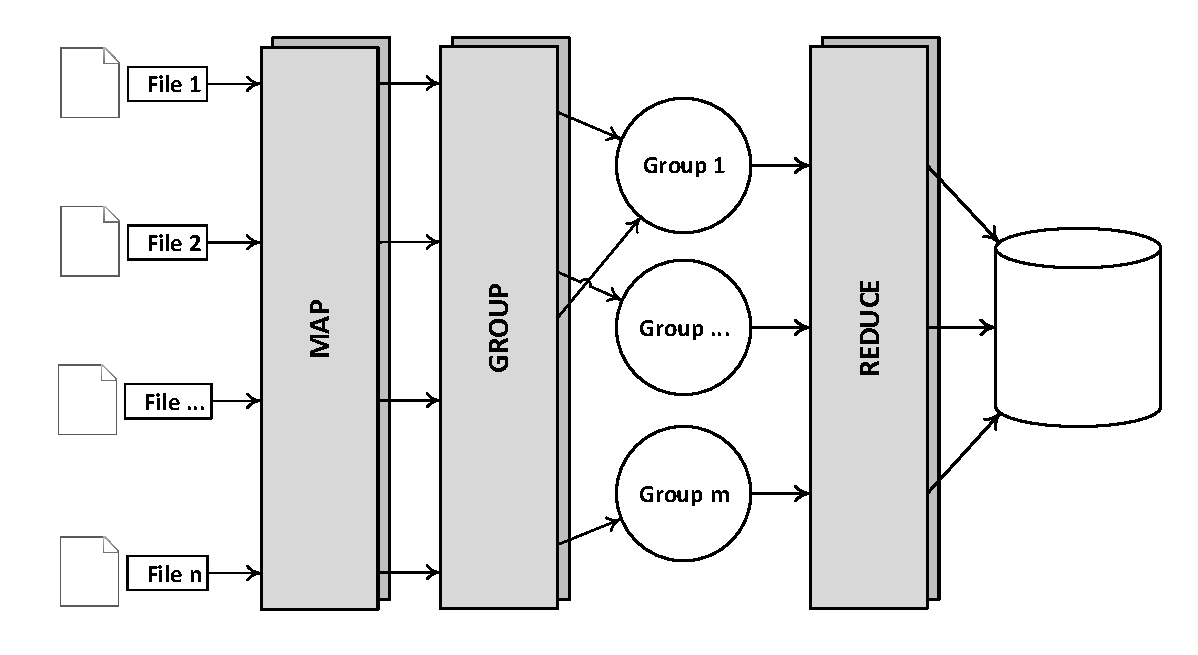
\includegraphics[height=.7\textheight]{mapred.pdf}
\end{figure}
\end{frame}

\begin{frame}
\frametitle{Logische Struktur II}
\begin{figure}
\centering
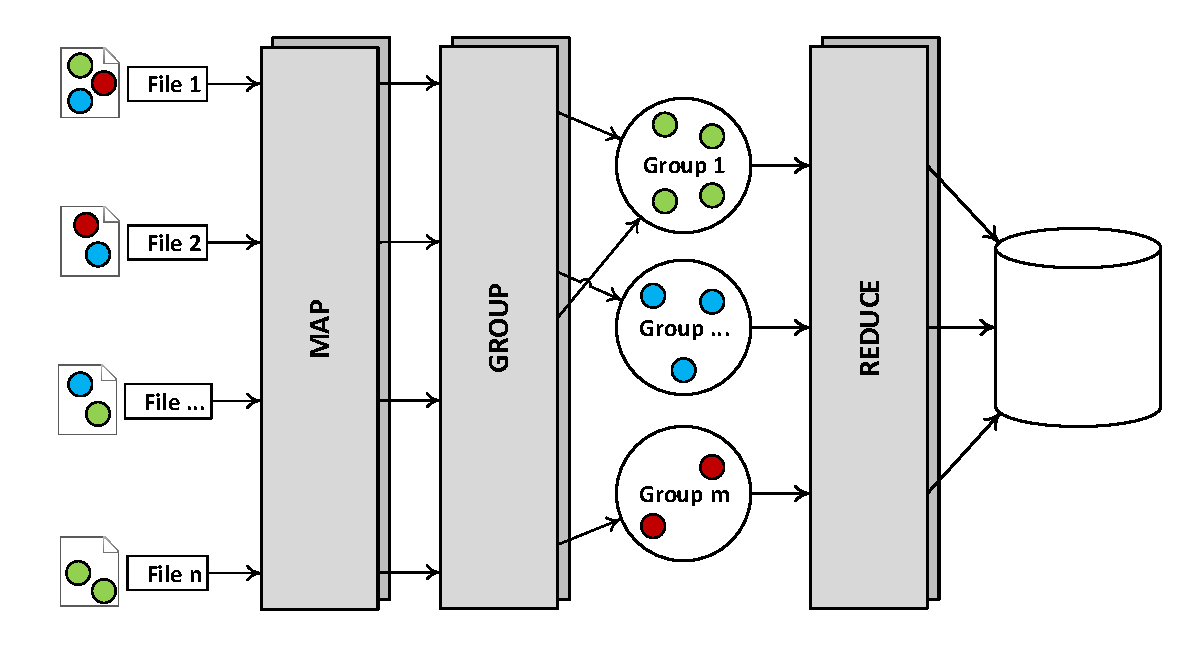
\includegraphics[height=.7\textheight]{mapred_groups.pdf}
\end{figure}
\end{frame}

%------------------------------------------------

\begin{frame}
\frametitle{Funktionsblöcke}
    \begin{enumerate}
    \setlength\itemsep{1em}
    \item \textbf{Map}    = Parsen der Textdateien
    \item \textbf{Group}  = Sortieren der Datenstrukturen nach Schlüssel
    \item \textbf{Reduce} = Summieren der Aggregationsfelder
    \end{enumerate}
\end{frame}

%------------------------------------------------
\section{Parallelrechner}

\begin{frame}
\tableofcontents[currentsection]
\setcounter{subsection}{1}
\end{frame}
%------------------------------------------------

\begin{frame}
\frametitle{Flynnsche Klassifizierung}
    \citeauthor{flynn1966very} (\citeyear{flynn1966very}) unterteilt Rechner nach ihrer Prozessoranzahl und den von ihnen gesteuerten Kontroll- und Datenflüssen in vier Kategorien:
    \begin{itemize}
    \setlength\itemsep{1em}
    \item Single Instruction Stream--Single Data Stream (SISD)
    \item Single Instruction Stream--Multiple Data Stream (SIMD)
    \item Multiple Instruction Stream--Single Data Stream (MISD)
    \item Multiple Instruction Stream--Multiple Data Stream (MIMD)
    \end{itemize}
\end{frame}

\begin{frame}
\frametitle{Speicheraufbau}
\onslide<2->{
    \begin{block}{Zusammenhängender Speicher}
    Als Multiprozessoren, bzw. \textit{Shared Memory Machines (SMMs)}, werden Rechner bezeichnet, deren CPUs einen physikalisch gemeinsamen Speicher mit zusammenhängendem Adressraum besitzen.
    Die darin enthaltenen Daten stehen allen Prozessoren direkt zur Verfügung und können zwischen ihnen geteilt werden.
    (Vgl. \cite{rauber2012parallele}, S.20ff)
    \end{block}
}
\onslide<3->{
    \begin{block}{Verteilter Speicher}
    \textit{Distributed Memory Machines (DMMs)}, auch Multicomputer genannt, arbeiten mit einem physikalisch separierten Speicher, welcher dem jeweiligen lokalen Prozessor privat zur Verfügung steht.
    (Vgl. \cite{rauber2012parallele}, S.26)
    \end{block}
}
\end{frame}

\begin{frame}
\frametitle{Programmiermodell}
\onslide<2->{
    \begin{block}{Shared Memory}
    Aus dem gemeinsamen Zugriff aller Prozessoren auf dieselben Daten erwächst ein Bedarf nach Synchronisation.
    Dies geschieht durch das Prinzip des gegenseitigen Ausschlusses (engl.: \textit{Mutual Exclusion (Mutex)}).
    Mutex-Objekte signalisieren Threads/Prozessen ob auf eine Ressource im Hauptspeicher zugegriffen werden darf.
    \end{block}
}
\onslide<3->{
    \begin{block}{Message Passing}
    Beim Message Passing verfügt jede CPU über ihre eigene Kopie der Daten.
    Werden für eine Berechnung Daten eines fremden Speicher-\newline
    bereichs benötigt, so müssen diese explizit durch Nachrichten angefordert und anschließend übertragen werden.
    \end{block}
}
\end{frame}

%------------------------------------------------
\section[Parallelisierung]{Möglichkeiten der Parallelisierung}

\begin{frame}
\tableofcontents[currentsection]
\end{frame}
%------------------------------------------------

\setcounter{subsection}{1}
\subsection{Haskell}

\begin{frame}
\frametitle{Die Haskell Laufzeitumgebung}
\onslide<2->{
    \begin{block}{Bedarfsauswertung}
    Bedarfsauswertung (engl.: \textit{lazy evaluation}) bezeichnet eine Evaluationsstrategie, bei der die Argumente einer Funktion erst dann ausgewertet werden, wenn sie tatsächlich benötigt werden.
    \end{block}
}

\onslide<3->{
    \begin{block}{Thunk}
    Ein Thunk ist eine unevaluierte Berechnungseinheit innerhalb eines Haskell Programms.
    \end{block}
}
\end{frame}

\begin{frame}[plain]{}
\begin{figure}
\centering
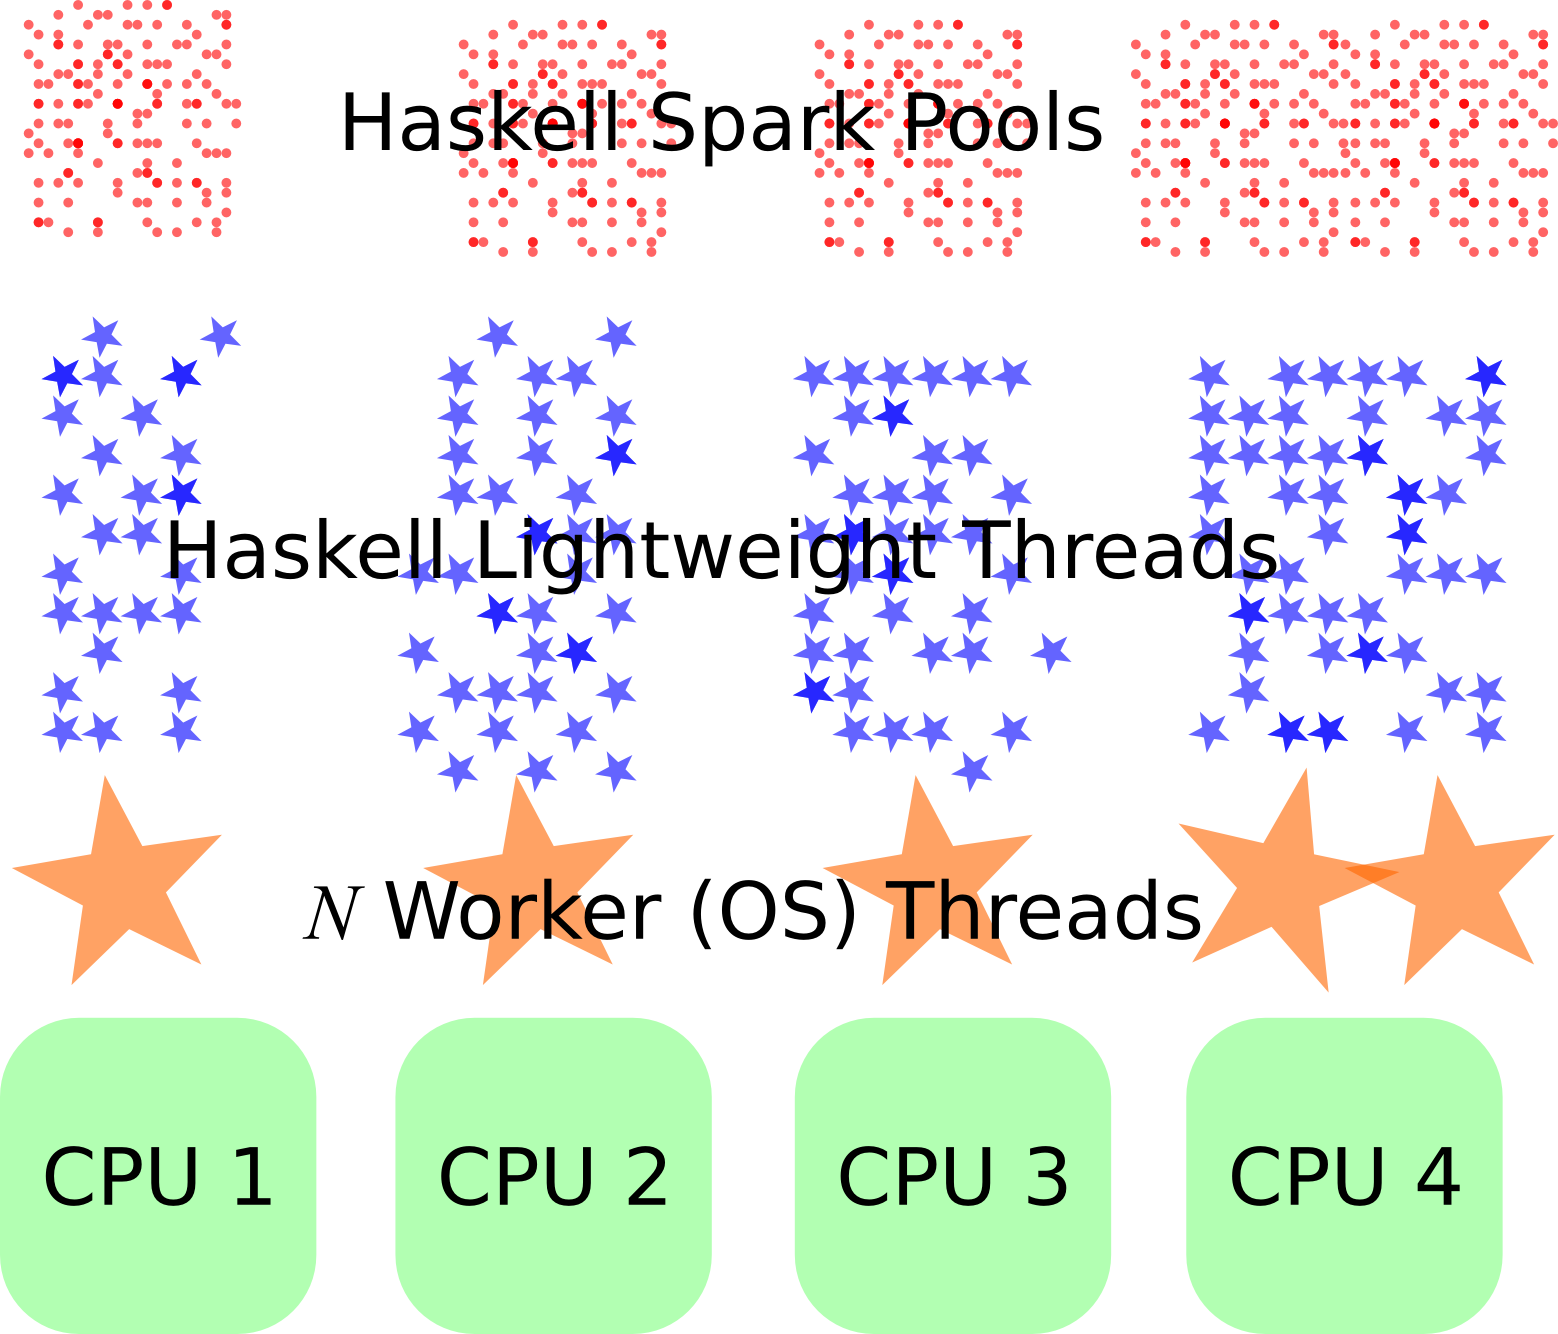
\includegraphics[height=.8\textheight]{sparks}
    \caption{Don Stewart (\href{https://stackoverflow.com/questions/958449/what-is-a-spark-in-haskell}{$\rightarrow$ Stackoverflow-Link})}
\end{figure}
\end{frame}

\begin{frame}
\frametitle{Parallele Kombinatoren I}
    \citeauthor{trinder1998algorithm} (\citeyear{trinder1998algorithm}) definiert folgende zwei Kombinatoren:
    \begin{itemize}
    \setlength\itemsep{1em}
        \onslide<1->{
            \item {\color{blue}\texttt{x `par` y}} kreiert einen potentiell parallelen Thunk (=Spark) für das Argument \texttt{x} und gibt anschließend \texttt{y} zurück
            \item {\color{blue}\texttt{x `pseq` y}} sorgt für die Auswertung von \texttt{x} bevor \texttt{y} zurückgegeben wird
        }
        \onslide<2->{
            \item[$\rightarrow$] {\color{blue}\texttt{x `par` y `pseq` f x y }}
        }
    \end{itemize}
\end{frame}

\begin{frame}
\frametitle{Parallele Kombinatoren II}
    \citeauthor{marlow2010seq} (\citeyear{marlow2010seq}) definieren neue Formen dieser Kombinatoren:
    \begin{itemize}
        \item {\color{blue}\texttt{r0 x}} = führe keinerlei Evaluation von \texttt{x} aus
        \item {\color{blue}\texttt{rpar x}} = generiere einen Spark für \texttt{x}
        \item {\color{blue}\texttt{rseq x}} = evaluiere \texttt{x} bis zu seinem Konstruktor
        \item {\color{blue}\texttt{rdeepseq x}} = evaluiere \texttt{x} vollständig
    \end{itemize}
    \bigskip
    Diese Funktionen geben eine Version ihres Argumentes zurück,\\in der die \underline{Evaluationsstrategie eingebettet} ist.
\end{frame}

\begin{frame}[plain]{}
\begin{figure}
\centering

\includegraphics[height=.7\textheight]{but_why}
\end{figure}
\end{frame}

\begin{frame}[fragile]
    \frametitle{Typspezifische Strategien}
    \begin{lstlisting}[language=haskell]
    evalList :: Strategy a -> Strategy [a]
    evalList s []     = return []
    evalList s (x:xs) = do x' <- s x
                        xs'   <- evalList s xs
                        return (x':xs')
    \end{lstlisting}
\end{frame}

\begin{frame}[fragile]
    \frametitle{Algorithmus + Strategie}
    \begin{lstlisting}[language=haskell,otherkeywords={using}]
    map f [1,2,...] `using` (evalList rpar)
    \end{lstlisting}
\end{frame}

\begin{frame}
\frametitle{Evaluationsstrategien}
    \begin{itemize}
        \item[+] Separation von Algorithmus und Strategie
        \item[+] Typspezifische Strategien
        \item[$\sim$] Nur geeignet für ,,lazy'' Datenstrukturen
        \item[--] Hoher Komplexitätsgrad
    \end{itemize}
\end{frame}

\begin{frame}
\frametitle{Par Monade}
    \begin{itemize}
    \item Explizite Erstellung paralleler Kontrollflüsse, ähnlich Kindprozessen
    \item Synchronisation und Datenaustausch über \texttt{IVars} ($\sim$ Futures)
    \item Grundlegende Funktionen:
        \begin{itemize}
            \item \texttt{fork :: Par () -> Par ()}
            \item \texttt{put  :: NFData a => IVar a -> a -> Par ()}
            \item \texttt{get  :: IVar a -> Par a}
        \end{itemize}
    \end{itemize}
\end{frame}

\begin{frame}
\frametitle{Par Monade}
    \begin{itemize}
        \item[+] Explizite Kontrolle über Parallelität
        \item[$\sim$] Vorrangig für Strukturen der Typklasse \texttt{NFData} gedacht
    \end{itemize}
\end{frame}

%------------------------------------------------

\subsection{C++}

\begin{frame}
\frametitle{Manuelle Parallelisierung I}
    \onslide<2->{
        \textbf{POSIX-Threads (PThreads)}
        \begin{itemize}
            \item IEEE POSIX 1003.1c standard (1995)
            \item Implementierung des Threadmodells für POSIX-Systeme
            \item Prozeduren enthalten in Headerdatei \texttt{pthread.h}
        \end{itemize}
    }

    \vfill

    \onslide<3->{
        \textbf{std::threads}
        \begin{itemize}
            \item Modernere Alternative (seit \C++11) in Form einer Standardbibliothek
            \item Synchronisation z.B. mittels \texttt{std::mutex} Komponenten
        \end{itemize}
    }
\end{frame}

\begin{frame}
\frametitle{Manuelle Parallelisierung II}
    \begin{itemize}
        \item[+] Größtmögliche Flexibilität
        \item[--] \textbf{Aufwending}
    \end{itemize}
\end{frame}

\begin{frame}
\frametitle{Parallele APIs I}
    \textbf{Open Multiprocessing (OpenMP)}
    \begin{itemize}
        \item Seit 1997 in Zusammenarbeit mehrerer namhafter Hardware- und Compilerhersteller entwickelt
        \item ,,[M]it dem Ziel [\dots], einen einheitlichen Standard für die Programmierung von Parallelrechnern mit gemeinsamen Adressraum zur Verfügung zu stellen'' (\cite{rauber2012parallele}, S.357)
        \item Pragma-Anweisungen, die für andere Compiler aussehen, wie Kommentare
        \item Vorrangig für Loop-Level Parallelisierung eingesetzt
    \end{itemize}
\end{frame}

\begin{frame}[fragile]
    \frametitle{Parallel for}
    \begin{lstlisting}[language=c,otherkeywords={pragma,for,parallel,omp}]
    #pragma omp parallel for
    for (i = 0; i < 10; ++i) {
        /* ... */
    }
    \end{lstlisting}
\end{frame}

\begin{frame}
\frametitle{Parallele APIs II}
    \begin{itemize}
        \item[+] Einfach und intuitiv
        \item[--] Weniger flexibel (Loop-Level, parallele Regionen)
        \bigskip
        \item Auch interessant:
            \begin{itemize}
            \item Intel Threading Building Blocks (TBB)
            \item Open Accelerator (OpenACC)
            \item Open Message Passing Interface (OpenMPI)
            \end{itemize}
    \end{itemize}
\end{frame}

\begin{frame}
\frametitle{Parallele Standardbibliotheken}
    \begin{itemize}
        \item Parallelität in vielen Funktionalen ist offensichtlich!
        \item \citeauthor{singler2007mcstl} (\citeyear{singler2007mcstl}, S.1) bezeichnen sie als ,,Embarrassingly parallel'', entwickelten parallele Versionen einiger Standardfunktionen
        \item Inklusive dynamischer Lastverteilung
        \item Basierend auf OpenMP
        \item Namespace \texttt{std::\_\_parallel}
    \end{itemize}
\end{frame}

\begin{frame}[fragile]
    \begin{lstlisting}[language=c]
    # include <parallel/algorithm>
    # include <parallel/numeric>
    namespace par = std::__parallel;

    par::transform( ... );  /* Map    */
    par::accumulate( ... ); /* Reduce */
    \end{lstlisting}
\end{frame}

\begin{frame}[plain]{}
\begin{figure}
\centering

\includegraphics[height=.7\textheight]{suspiciously_easy}
\end{figure}
\end{frame}

%------------------------------------------------
\section{Leistungskriterien}

\begin{frame}
\tableofcontents[currentsection]
\end{frame}
%------------------------------------------------

\setcounter{subsection}{1}
\subsection{Allgemeine Leistungskriterien}

\begin{frame}
\frametitle{Antwortzeit}
    \begin{block}{Definition}
    Die Antwortzeit $T_A$ (engl.: \textit{wallclock time}) eines Programms ist definiert als die Differenz zwischen Start seiner Ausführung und Beendigung seines letzten Prozesses, wie gemessen von einer herkömmlichen Wanduhr.
    \end{block}
\end{frame}

\begin{frame}
\frametitle{Durchschnittlich genutzter Arbeitsspeicher}
    \begin{block}{Definition}
    Die \textit{Resident Set Size (RSS)} entspricht dem belegten Bereich im Hauptspeicher der Maschine zu einem gegebenen Zeitunkt. Eventuell auf die Swap-Partition ausgelagerte Teile des Programms fließen nicht in den Wert ein.
    \end{block}
\end{frame}

\begin{frame}
\frametitle{Durchsatz}
    \begin{block}{Definition}
    Der Durchsatz $D(N)$ ist in vorliegendem Szenario definiert als die Anzahl verarbeiteter Datensätze $N$ pro Sekunde:
    $$D(N) = \frac{N}{T_A} [\text{Records/s}]$$
    \end{block}
\end{frame}

\begin{frame}
\frametitle{Cache Hit-Rate}
    \begin{block}{Definition}
    Der prozentuale Anteil der Read-Hits von der Gesamtzahl aller lesenden Cache-Zugriffe wird als Hit-Rate bezeichnet:
    $$\text{Hit-Rate} = \frac{\text{Read-Hits}}{\text{Read-Hits} + \text{Read-Misses}} [\%]$$
    \end{block}
\end{frame}

%------------------------------------------------

\subsection{Parallele Leistungskriterien}

\begin{frame}
\frametitle{Speedup}
    \begin{block}{Definition}
        Der Speedup $S(P)$ beschreibt, wie sehr ein paralleles Programm von einer steigenden Zahl zur Verfügung stehender CPUs profitiert:
        $$S_{rel}(P) = \frac{T_A(1)}{T_A(P)}$$
    \end{block}
\end{frame}

\begin{frame}
\frametitle{Effizienz}
    \begin{block}{Definition}
        Die Effizienz eines parallelen Programms ist definiert als das Verhältnis aus Speedup $S(P)$ und der Zahl Prozessoren $P$ (vgl. \cite{rauber2012parallele}, S.179):
    $$E(P) = \frac{S(P)}{P}$$
    \end{block}
\end{frame}

\begin{frame}
\frametitle{Kosten}
    \begin{block}{Definition}
    Die Kosten $C(P)$ eines parallelen Programms entsprechen der Arbeit, die von allen eingesetzten Prozessoren zur Ausführung des Algorithmus aufgebracht wurde. Sie ist das Produkt aus Antwort-\\
    zeit $T_A$ und der Zahl eingesetzter Prozessoren $P$ (vgl. \cite{rauber2012parallele}, S.176):
    $$C(P) = T_A \cdot P$$
    \end{block}
\end{frame}

\begin{frame}
\frametitle{Paralleler Overhead}
    \begin{block}{Definition}
    Der Parallele Overhead $O(P)$ eines Programms beschreibt den Mehraufwand, welcher aus der Erstellung, Koordination und Beendigung Thread- basierter Parallelität resultiert:
    $$O(P) = \frac{C(P) - T_A(1)}{C(P)} \cdot 100 [\%]$$
    \end{block}
\end{frame}

%------------------------------------------------
\section{Messergebnisse}

\begin{frame}
\tableofcontents[currentsection]
\end{frame}
%------------------------------------------------

\setcounter{subsection}{1}

\begin{frame}
\frametitle{Speedup I}
    \begin{figure}
    \centering
    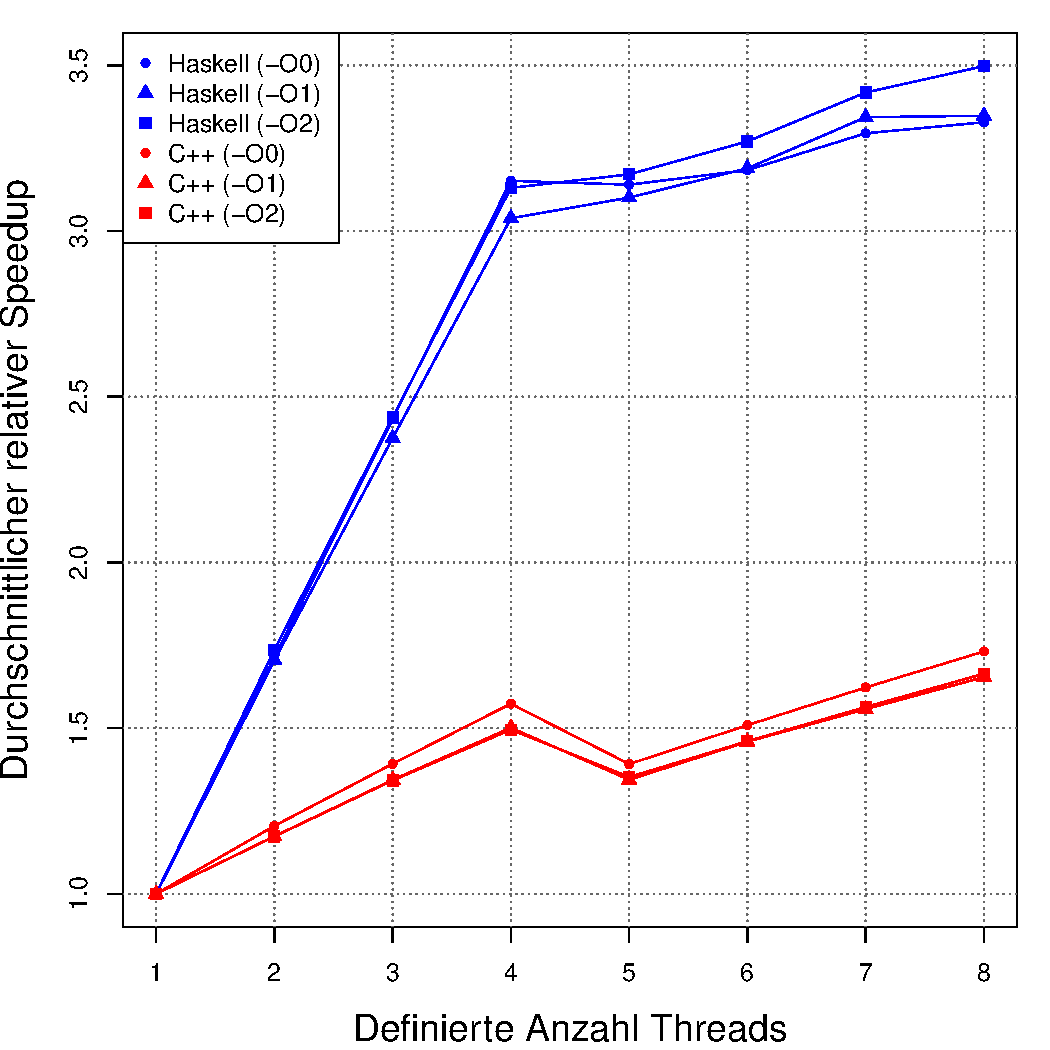
\includegraphics[height=.8\textheight]{speedup_desktop.pdf}
    \end{figure}
\end{frame}

\begin{frame}
\frametitle{Speedup II}
\begin{columns}[c]
\column{.5\textwidth}
    \begin{figure}
        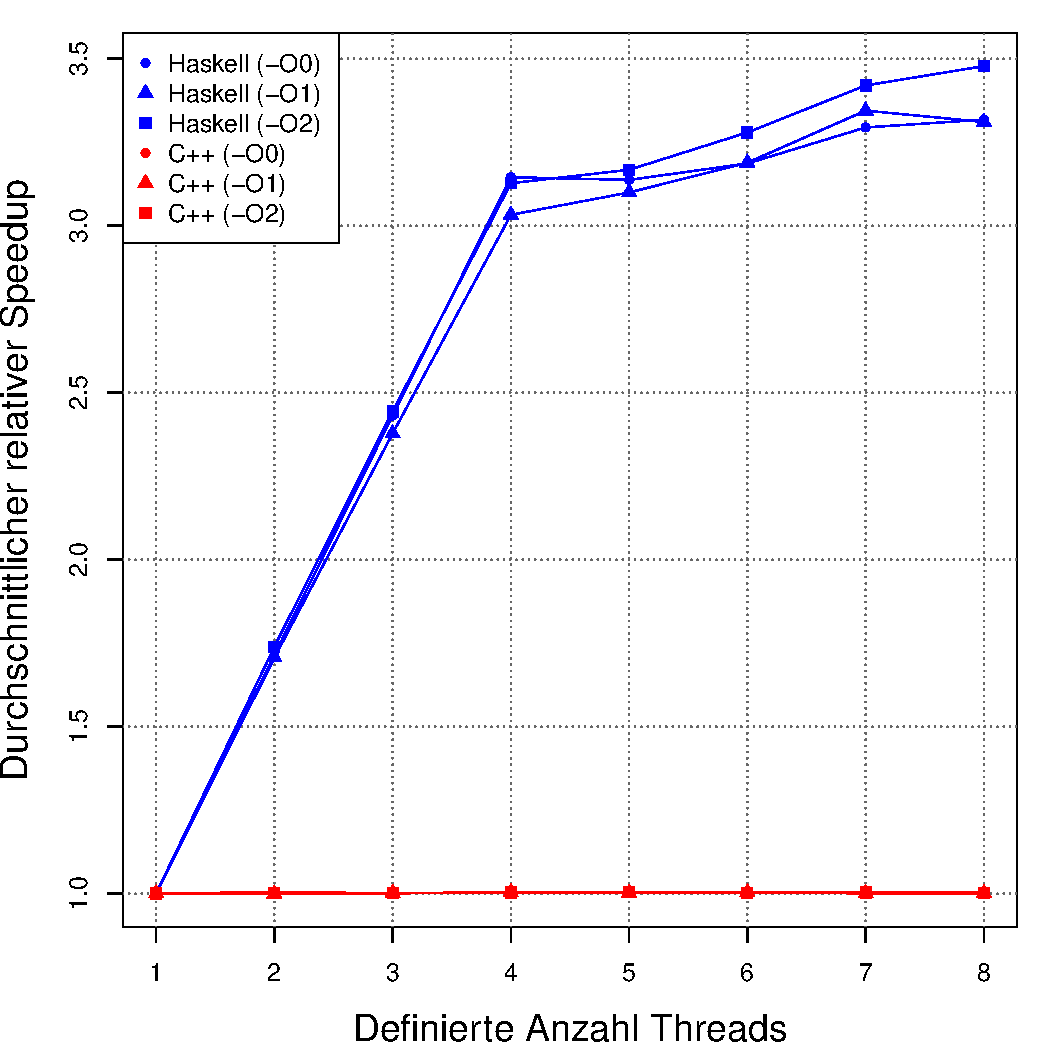
\includegraphics[width=\textwidth]{speedup_sub1000_desktop.pdf}
        \caption{< 1000 Dateien}
    \end{figure}

\column{.5\textwidth}
    \begin{figure}
        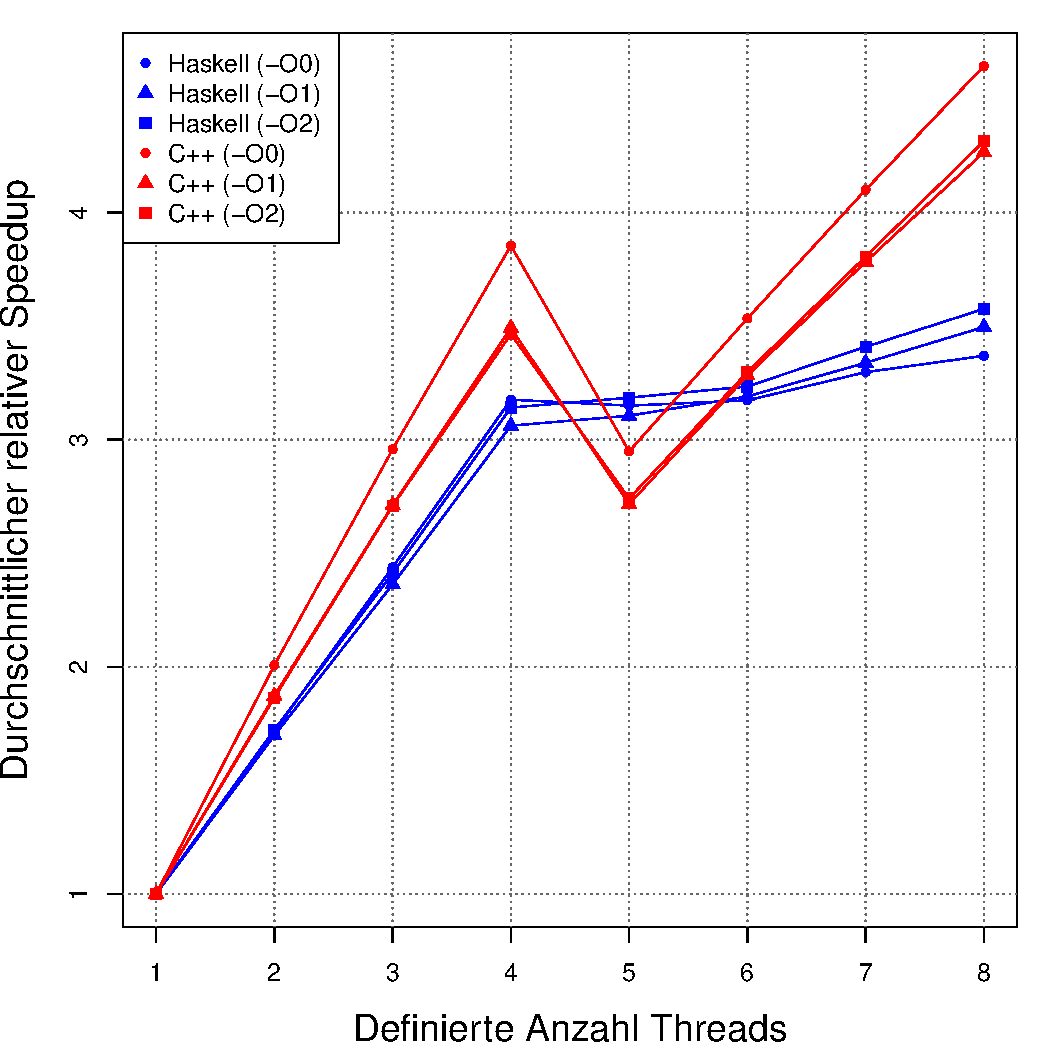
\includegraphics[width=\textwidth]{speedup_1000_desktop.pdf}
        \caption{1000 Dateien}
    \end{figure}
\end{columns}
\end{frame}

\begin{frame}
\frametitle{CPU Auslastung}
\begin{columns}[c]
\column{.5\textwidth}
    \begin{figure}
        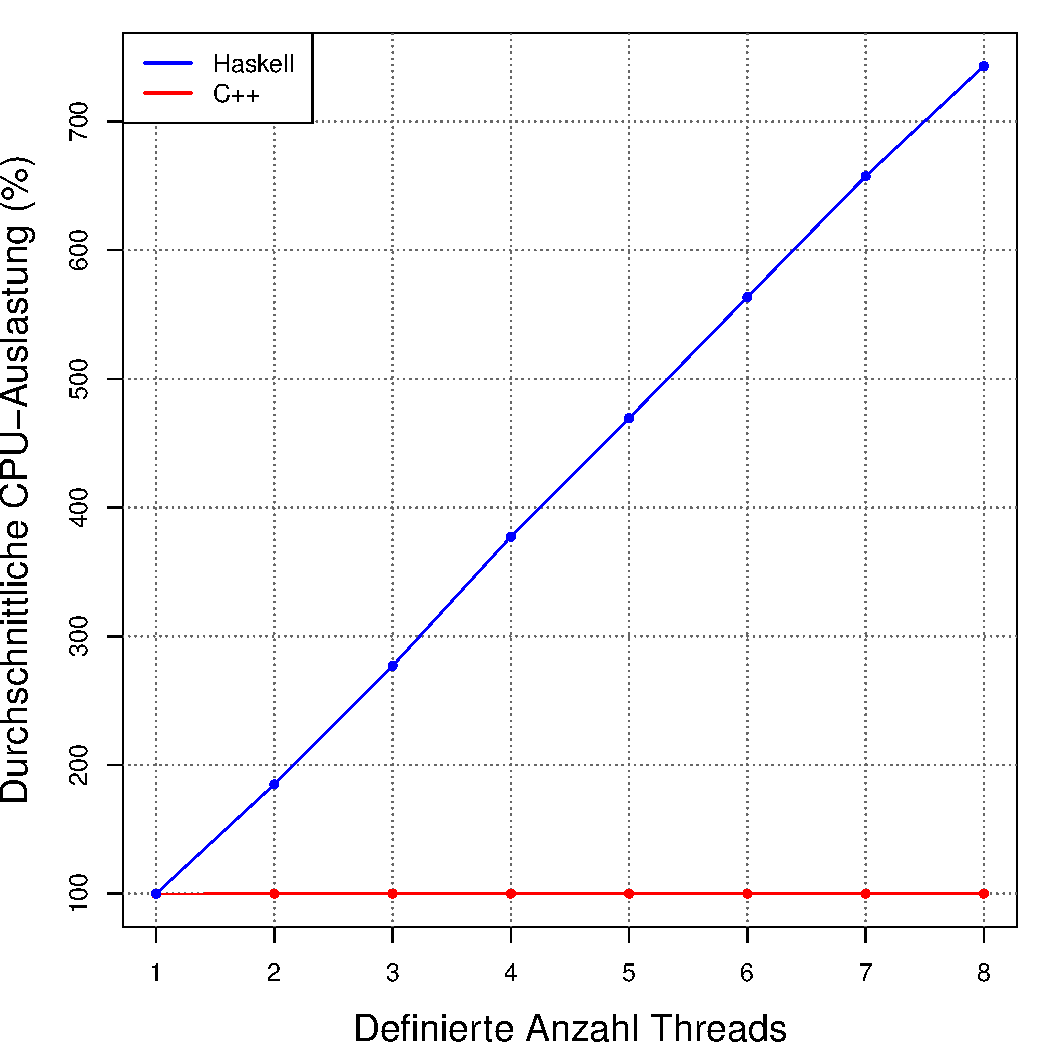
\includegraphics[width=\textwidth]{cpu_util_sub1000_desktop.pdf}
        \caption{< 1000 Dateien}
    \end{figure}

\column{.5\textwidth}
    \begin{figure}
        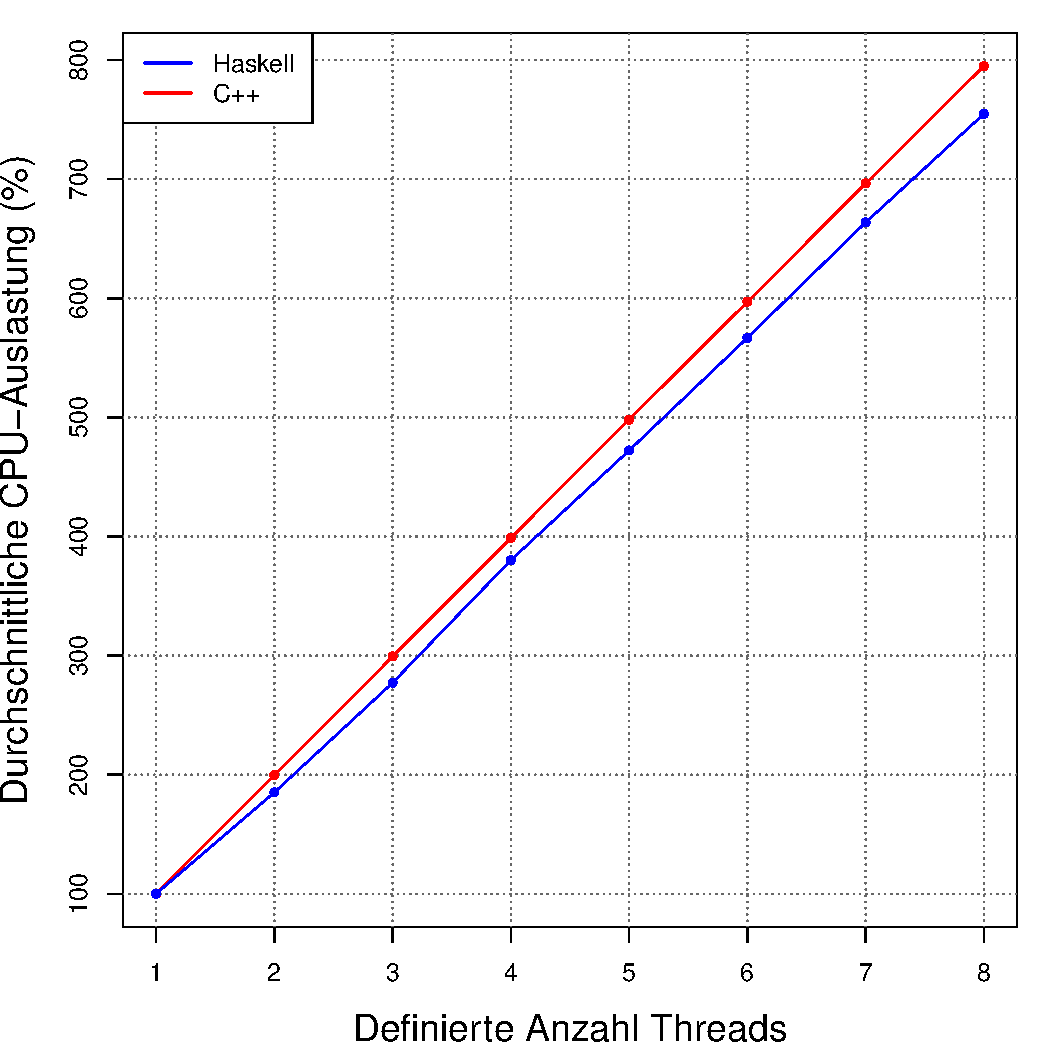
\includegraphics[width=\textwidth]{cpu_util_1000_desktop.pdf}
        \caption{1000 Dateien}
    \end{figure}
\end{columns}
\end{frame}

\begin{frame}
\frametitle{Effizienz}
\begin{columns}[c]
\column{.5\textwidth}
    \begin{figure}
        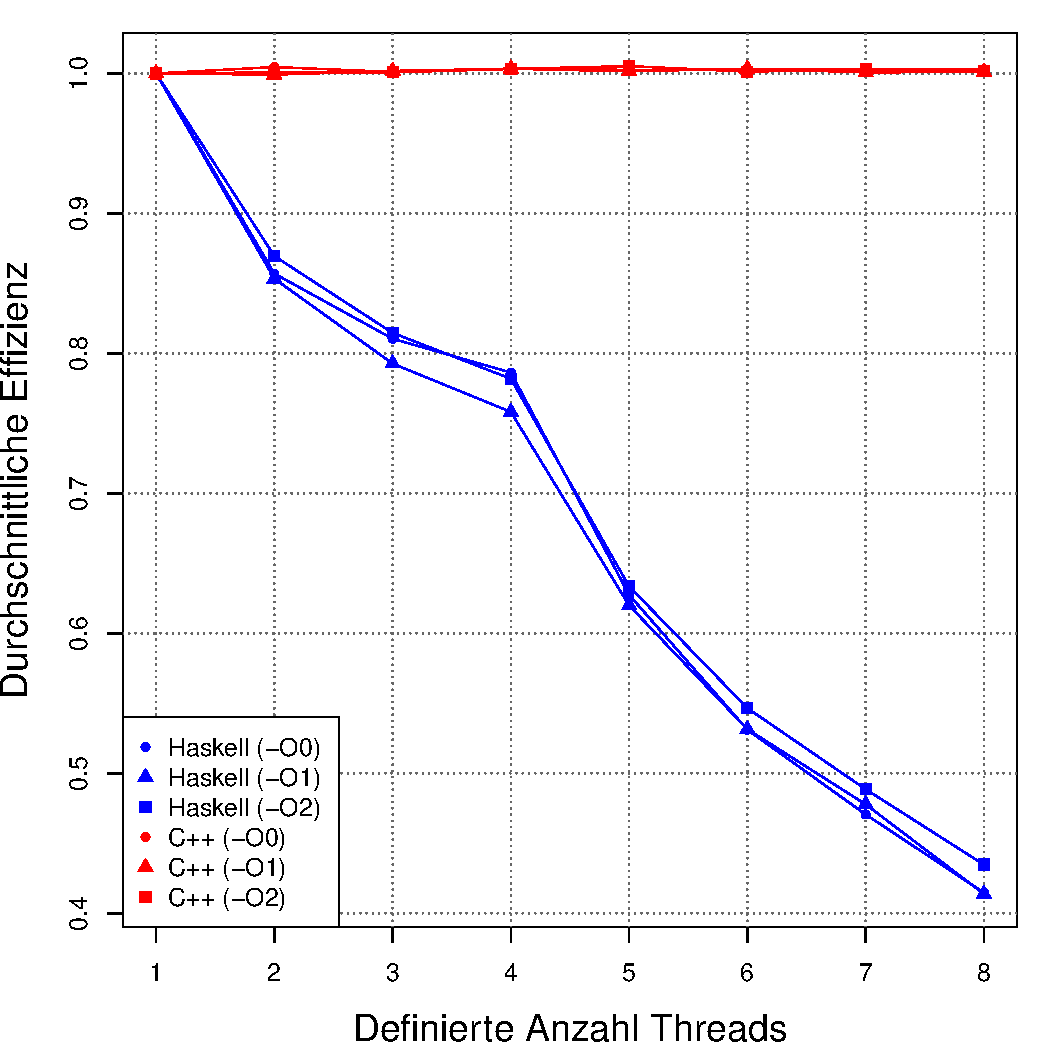
\includegraphics[width=\textwidth]{efficiency_sub1000_desktop.pdf}
        \caption{< 1000 Dateien}
    \end{figure}

\column{.5\textwidth}
    \begin{figure}
        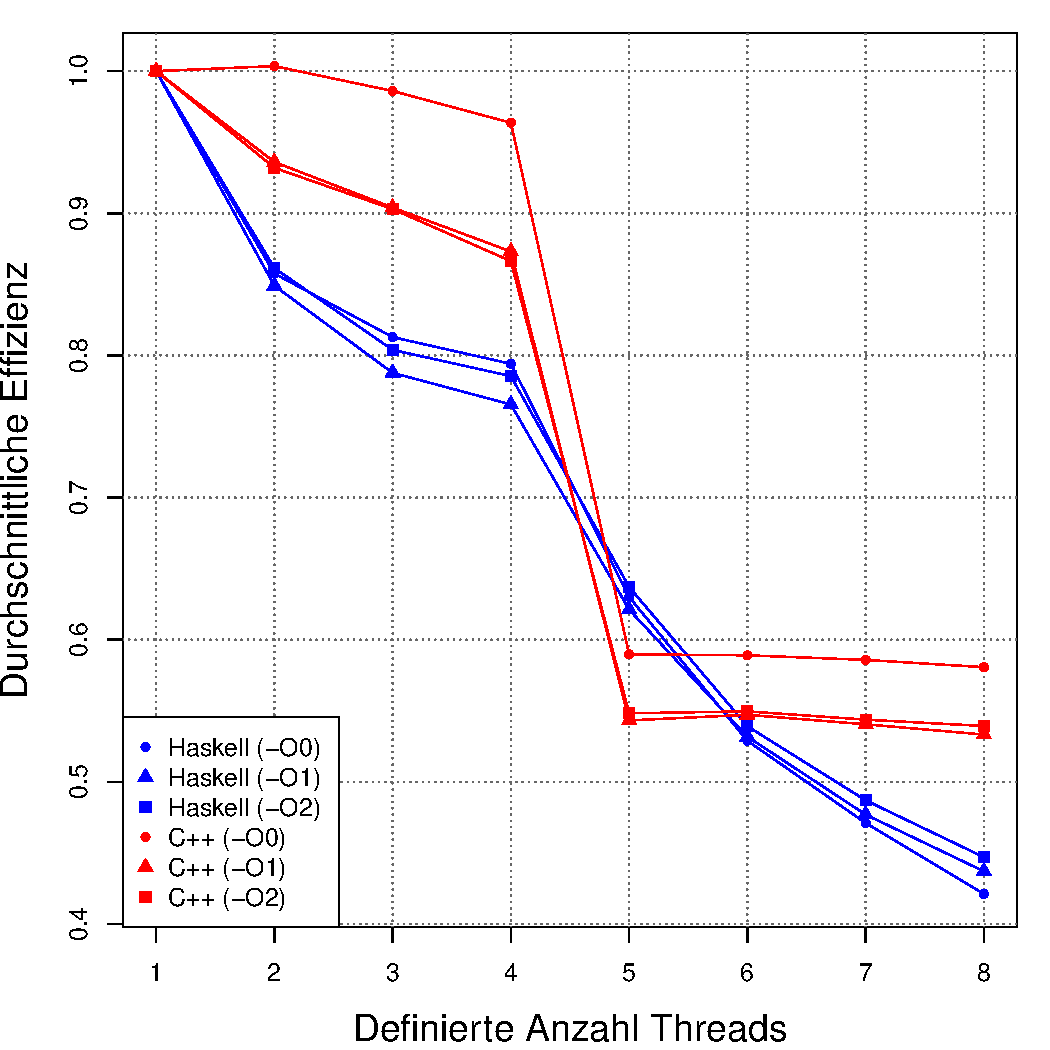
\includegraphics[width=\textwidth]{efficiency_1000_desktop.pdf}
        \caption{1000 Dateien}
    \end{figure}
\end{columns}
\end{frame}

\begin{frame}
\frametitle{Paralleler Overhead}
\begin{columns}[c]
\column{.5\textwidth}
    \begin{figure}
        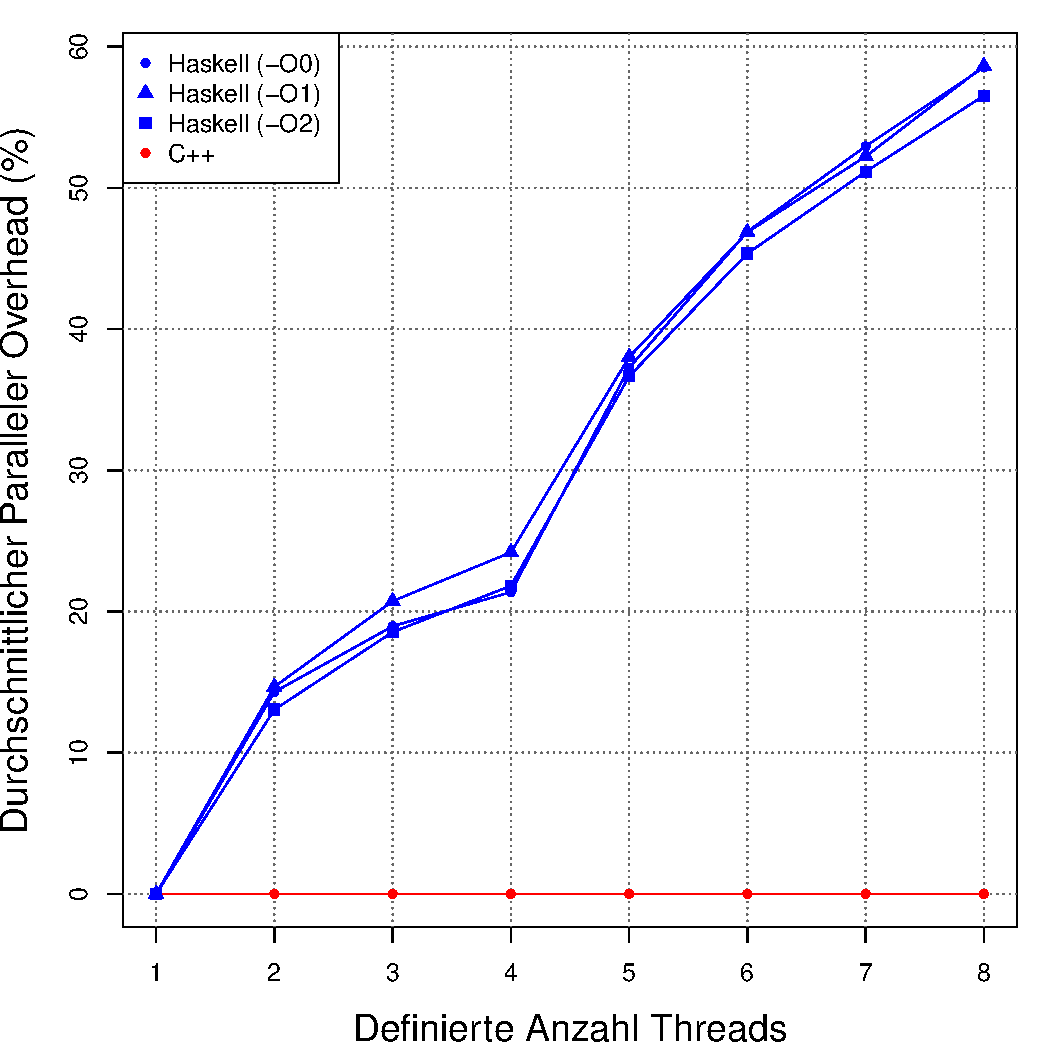
\includegraphics[width=\textwidth]{parallel_overhead_sub1000_desktop.pdf}
        \caption{< 1000 Dateien}
    \end{figure}

\column{.5\textwidth}
    \begin{figure}
        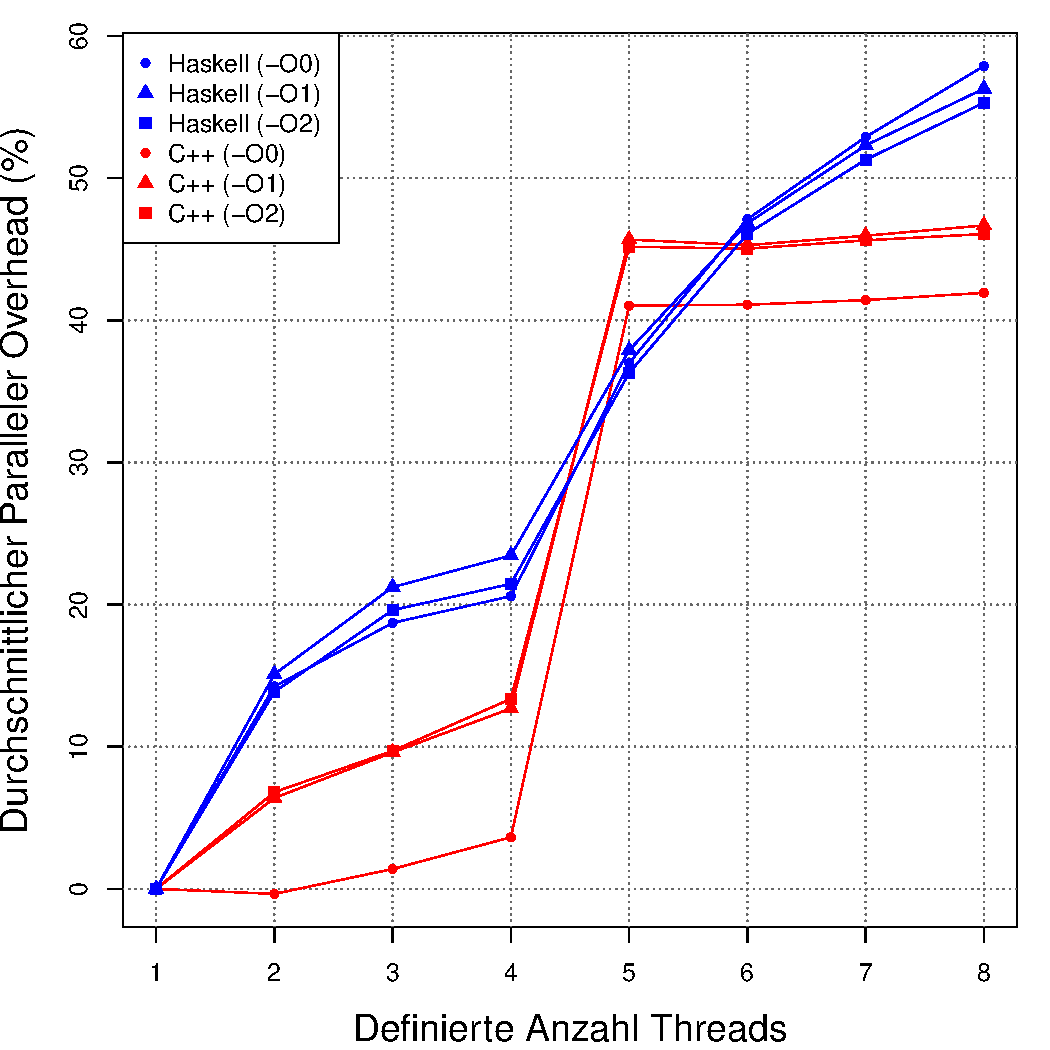
\includegraphics[width=\textwidth]{parallel_overhead_1000_desktop.pdf}
        \caption{1000 Dateien}
    \end{figure}
\end{columns}
\end{frame}

\begin{frame}
\frametitle{Kosten}
\begin{columns}[c]
\column{.5\textwidth}
    \begin{figure}
        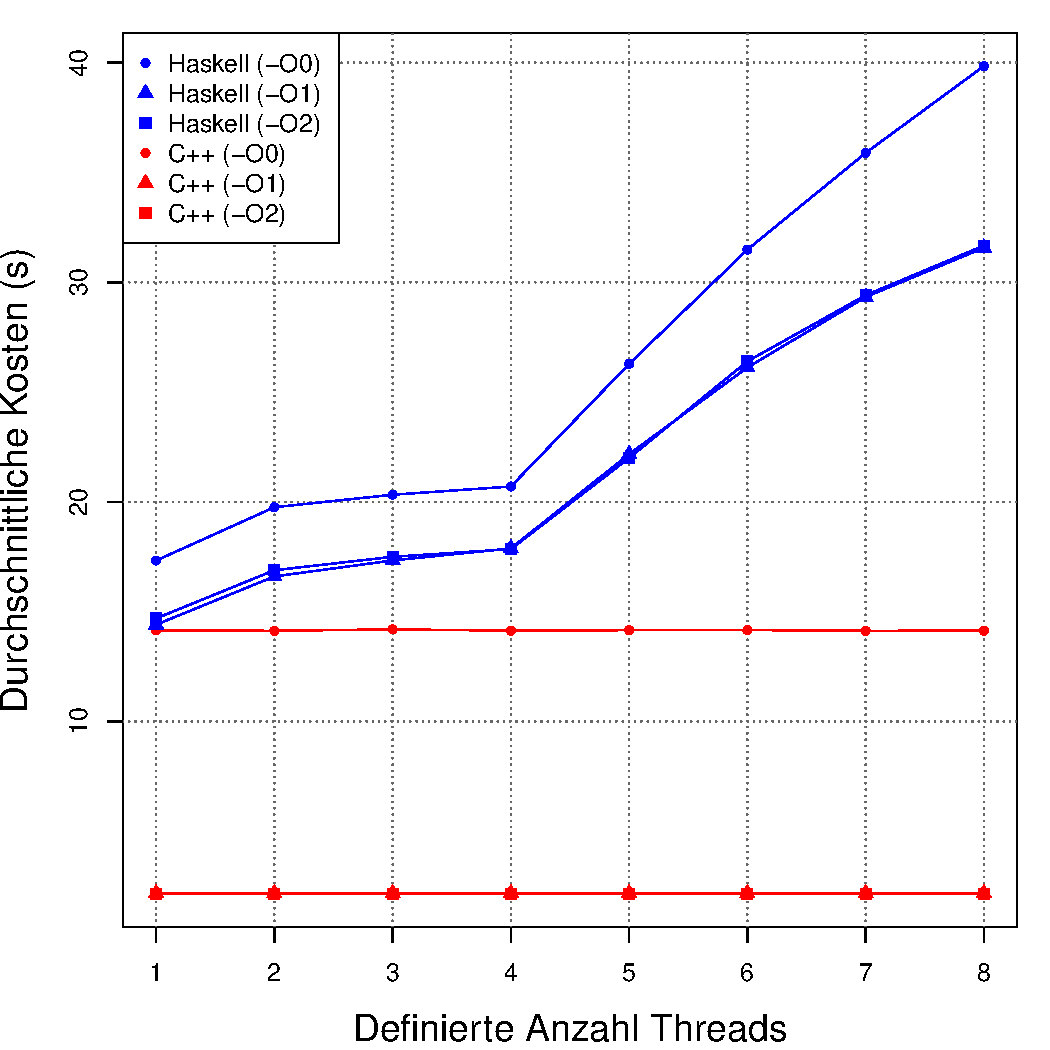
\includegraphics[width=\textwidth]{cost_sub1000_desktop.pdf}
        \caption{< 1000 Dateien}
    \end{figure}

\column{.5\textwidth}
    \begin{figure}
        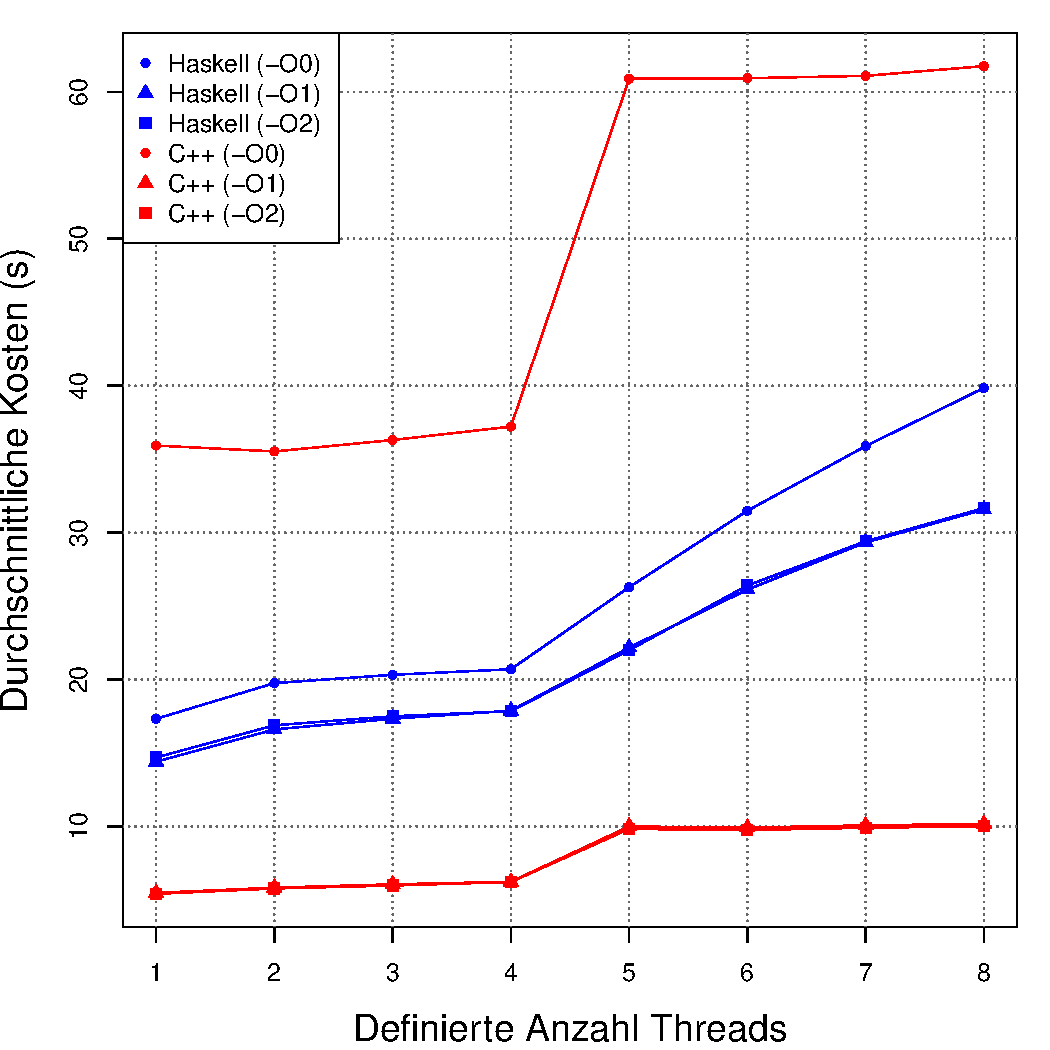
\includegraphics[width=\textwidth]{cost_1000_desktop.pdf}
        \caption{1000 Dateien}
    \end{figure}
\end{columns}
\end{frame}

\begin{frame}
\frametitle{Cache Hit-Rate}
    \begin{figure}
    \centering
    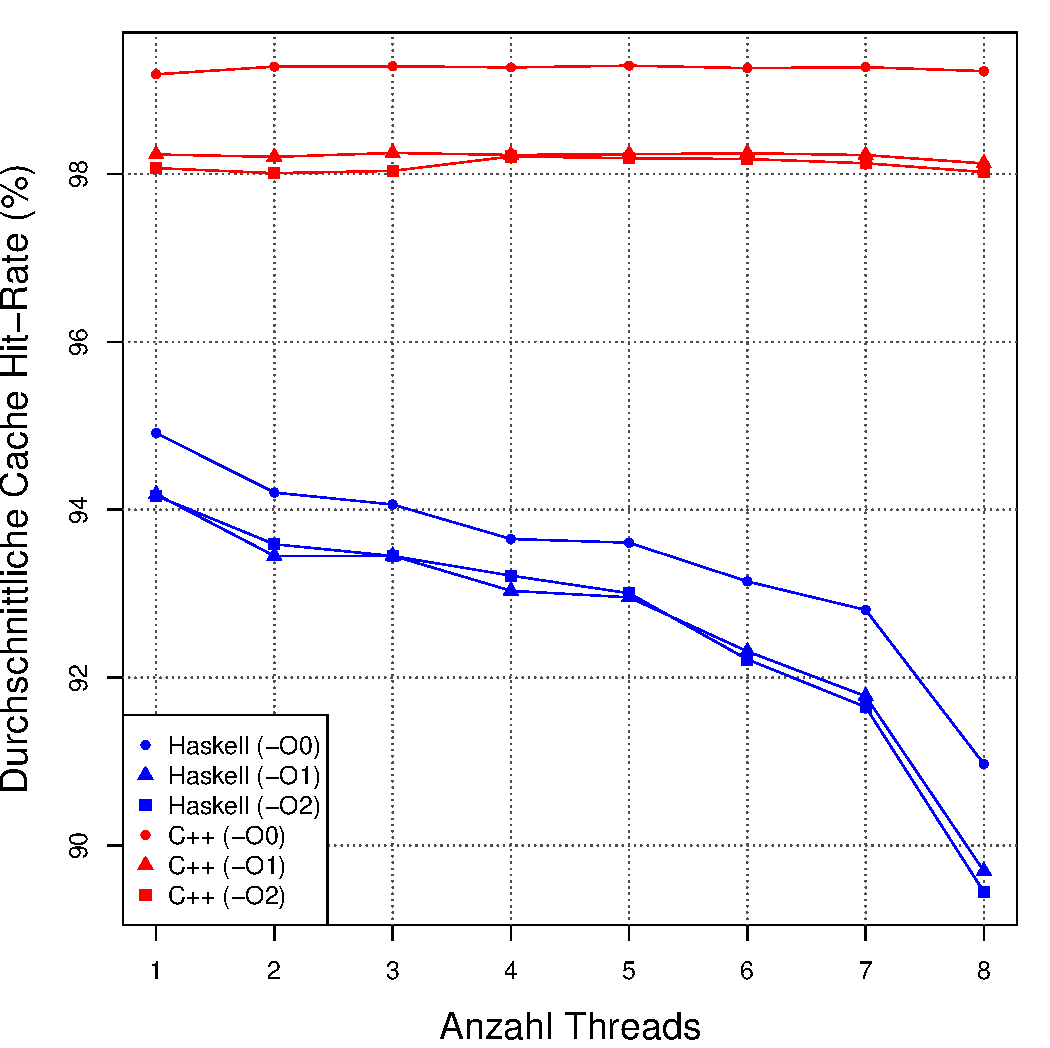
\includegraphics[height=.8\textheight]{cache_hit_rate.pdf}
    \end{figure}
\end{frame}

\begin{frame}
\frametitle{Durchsatz/Dateien}
\begin{columns}[c]
\column{.5\textwidth}
    \begin{figure}
        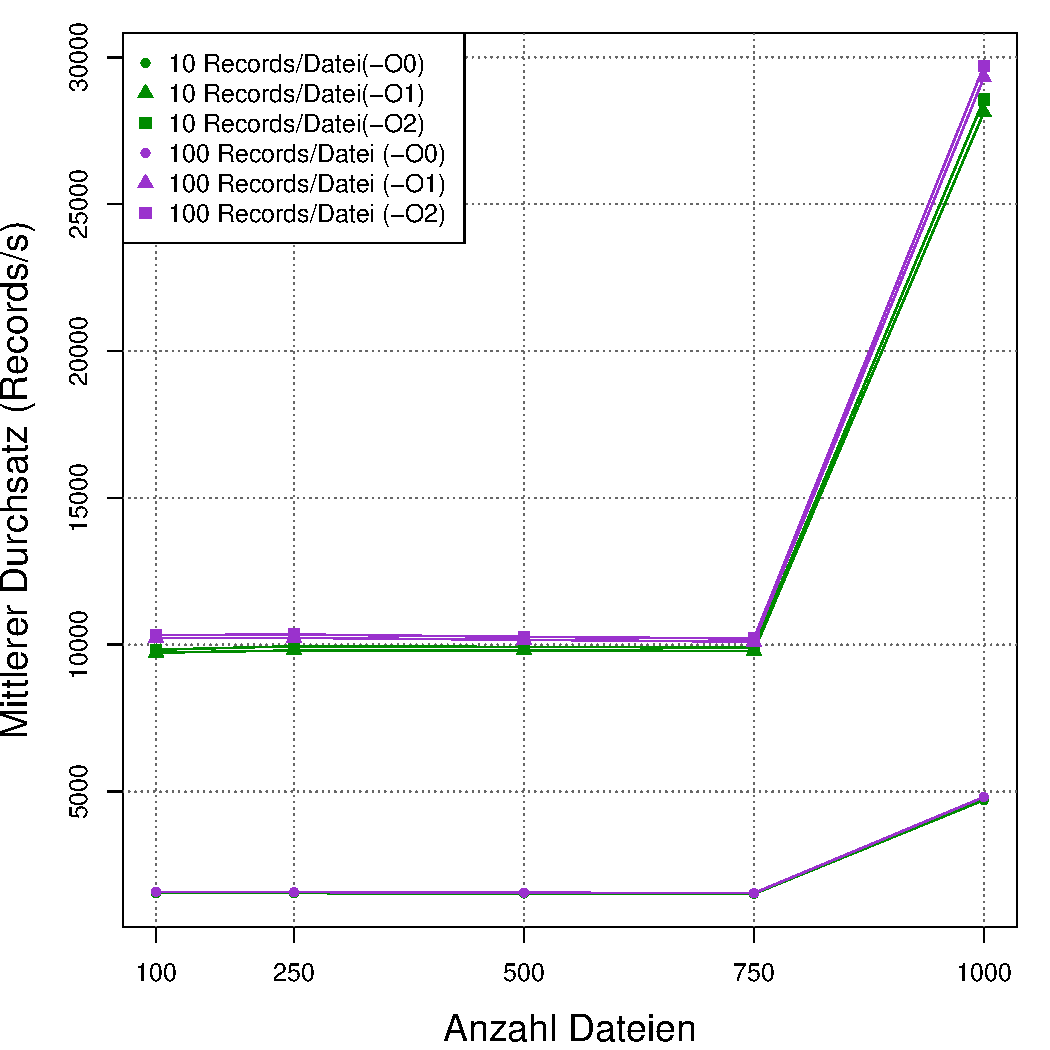
\includegraphics[width=\textwidth]{throughput_files_cpp_desktop.pdf}
        \caption{\C++}
    \end{figure}

\column{.5\textwidth}
    \begin{figure}
        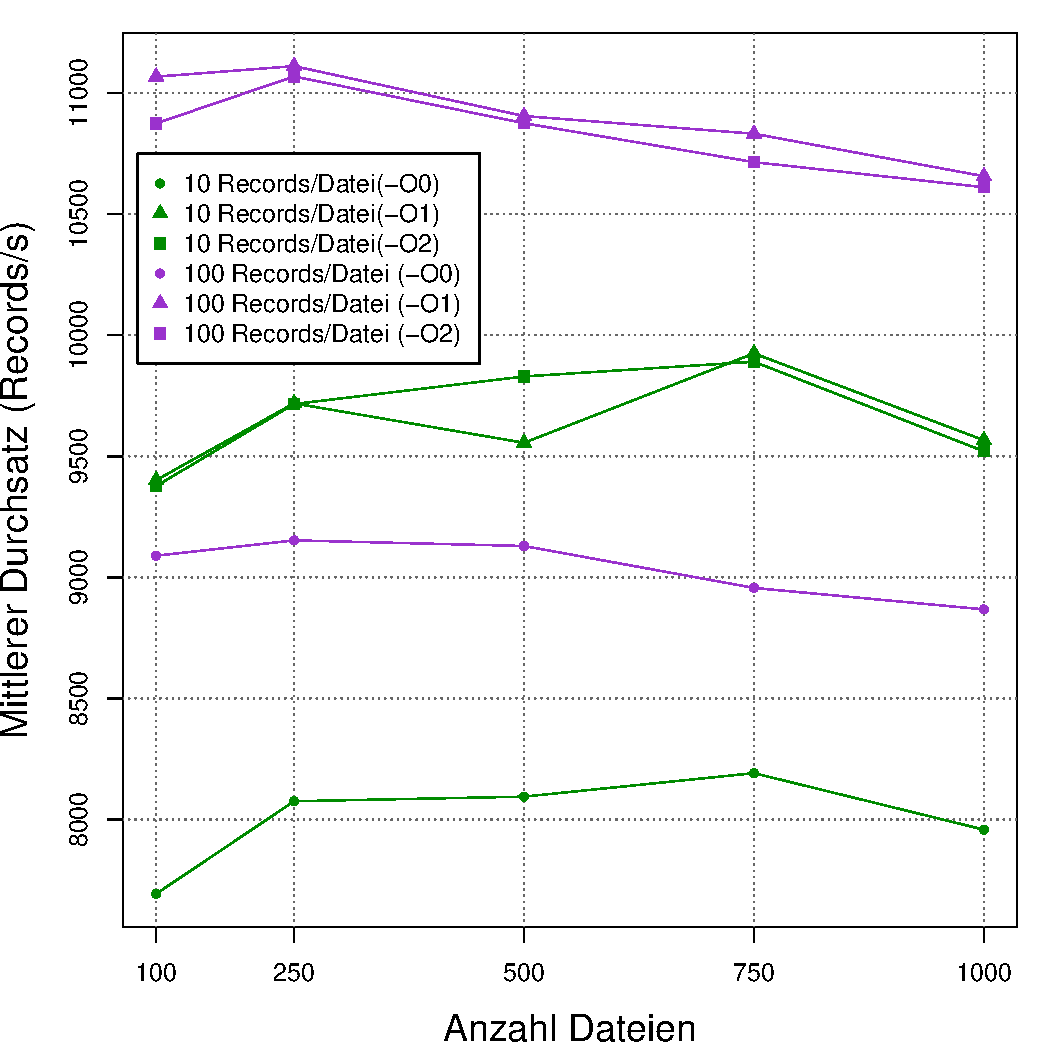
\includegraphics[width=\textwidth]{throughput_files_haskell_desktop.pdf}
        \caption{Haskell}
    \end{figure}
\end{columns}
\end{frame}

\begin{frame}
\frametitle{Durchsatz/Threads}
\begin{columns}[c]
\column{.5\textwidth}
    \begin{figure}
        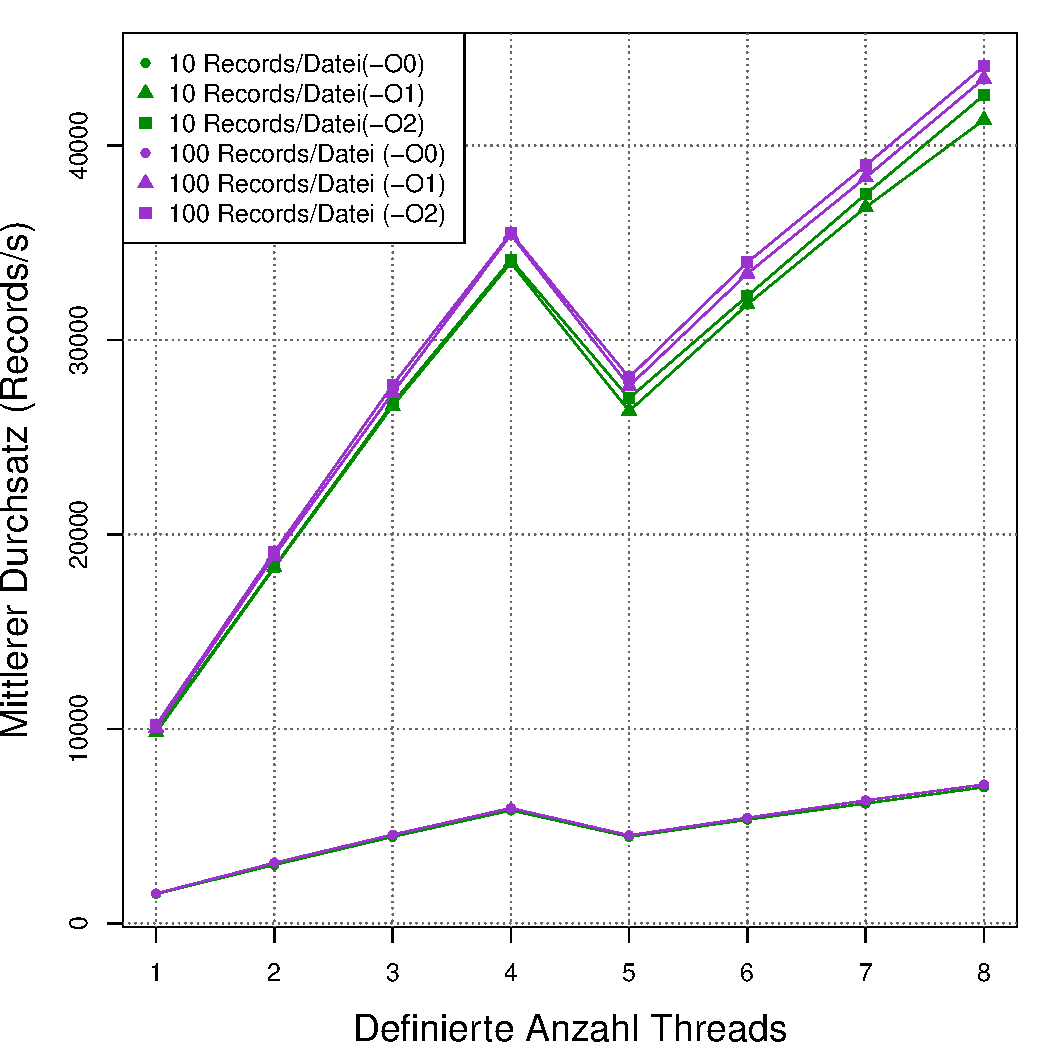
\includegraphics[width=\textwidth]{throughput_threads_1000_cpp_desktop.pdf}
        \caption{\C++}
    \end{figure}

\column{.5\textwidth}
    \begin{figure}
        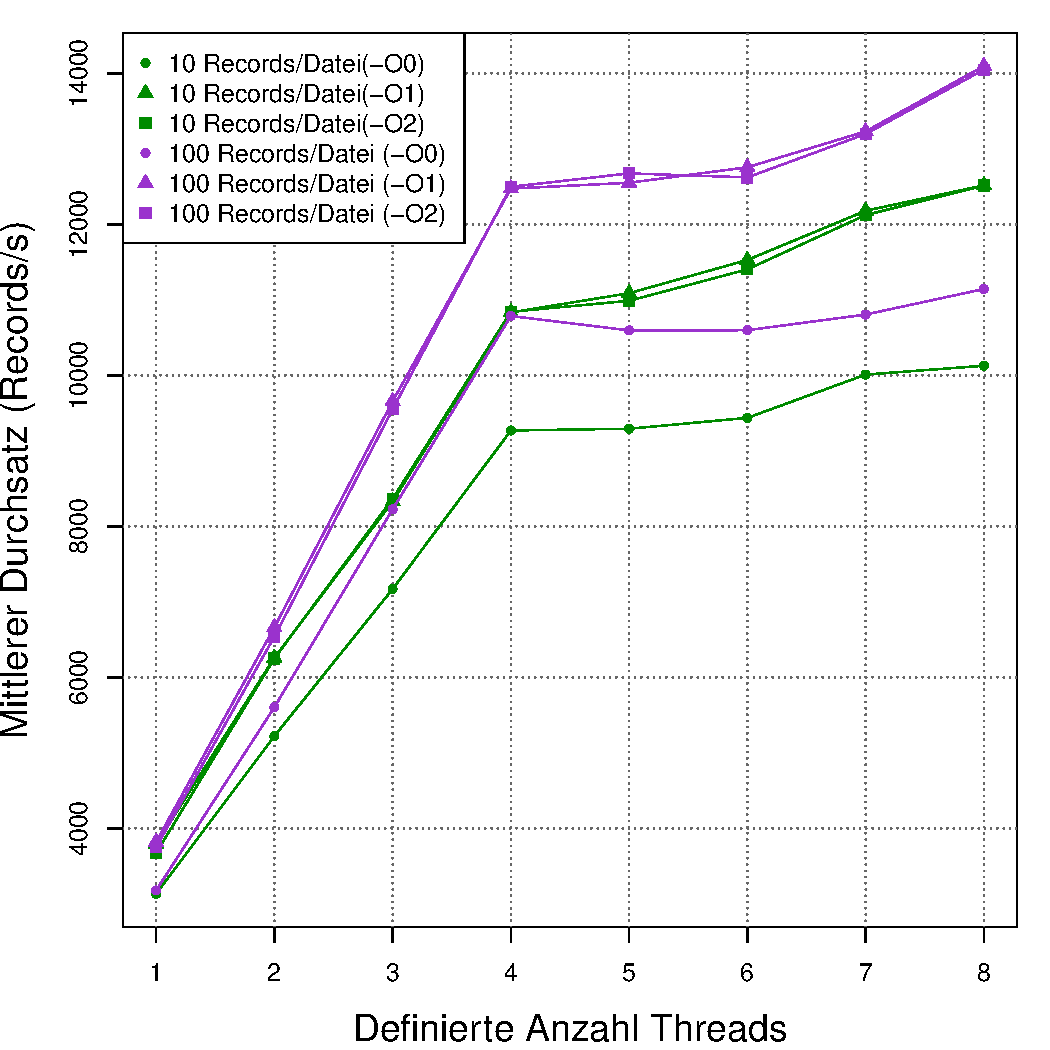
\includegraphics[width=\textwidth]{throughput_threads_1000_haskell_desktop.pdf}
        \caption{Haskell}
    \end{figure}
\end{columns}
\end{frame}

\begin{frame}
\frametitle{Durchschnittliche RSS}
    \begin{figure}
    \centering
    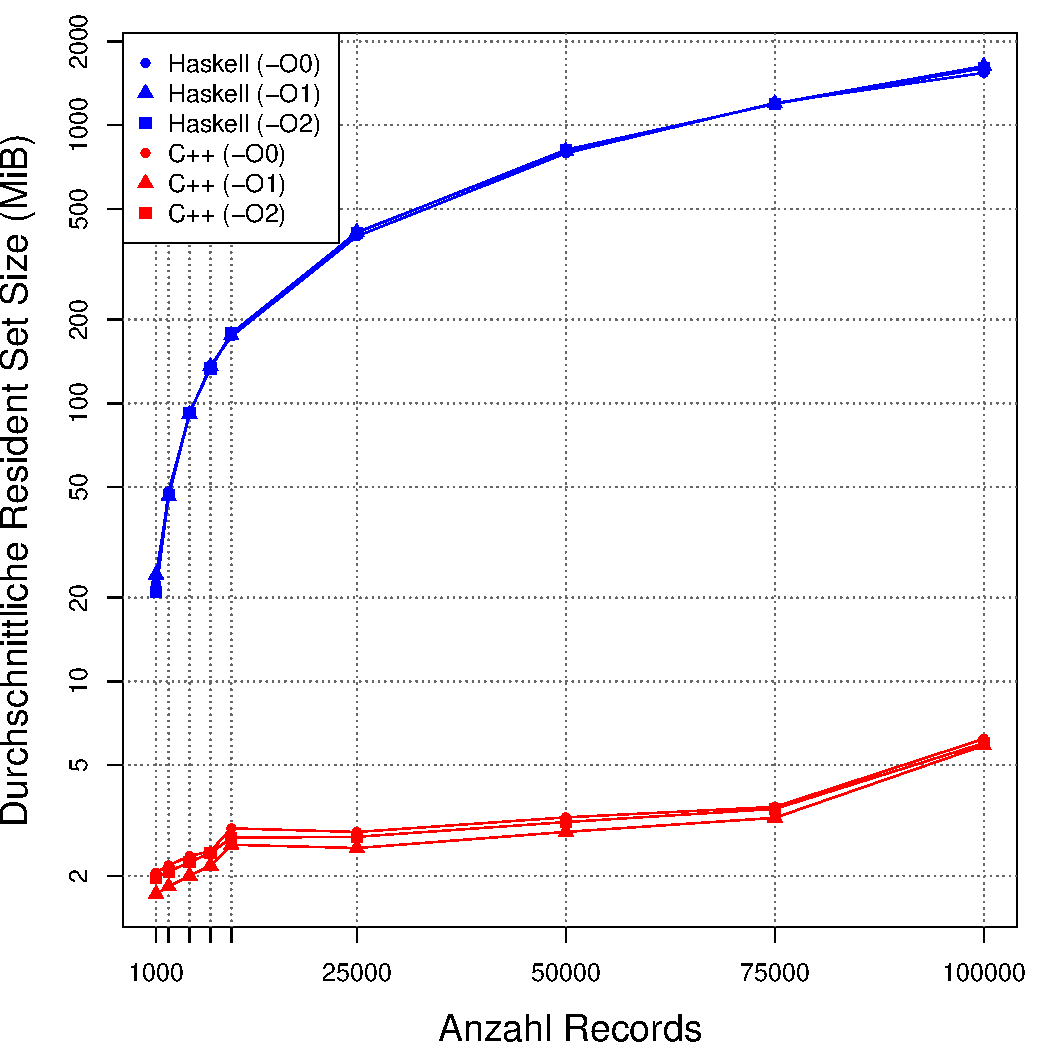
\includegraphics[height=.8\textheight]{average_rss_desktop.pdf}
    \end{figure}
\end{frame}

%------------------------------------------------
\begin{frame}
\centering
\Huge{Vielen Dank}
\end{frame}
%------------------------------------------------

\end{document} 
